\chapter{Cybercrime: Threat Landscape}
    Working on security we work on \textbf{risk}, which is composed of different elements:
    \begin{displaymath}
        Risk = Asset \times Vulnerabilities \times Threats
    \end{displaymath}
    The risk is the statistical and economical evaluation of the exposure to damage because of the presence of vulnerabilities and threats.\\
    With no threats there are no risks, because it is the only thing that can nullify this equation. Assets and vulnerabilities are never absent.\\
    With no \textit{Threat model} we're completely misguided on the management of our system in terms of security.
    \section{Threat landscape}
        Threats can be roughly divided along three directions:
        \begin{description}
            \item[Internal vs External treaths] an internal treath comes from the inside of the organization, it is part of the organization, while an external one don't.
            \item[Generic vs Targeted] many security threats are generic:
                \begin{itemize}
                    \item Generic threats: when you walk towards the underground, you're subjected to pickpocketers: they don't pick you because it's you, you're one of the others, it is a generic treath.
                    \\Generic threats are not linked to us by definition, they are linked to us because we look alike somebody easy to be pickpocketed, not because we were the target.
                    \item We can also consider also threats which are not so very generic: aggressions for sexual reasons are more targeted to one gender than one other, while still being generic.
                    \item Targeted threats: specifically designed against us: criminals target \textbf{that specific company} \textit{(e.g. the know how for racing cars, i want to steal from THAT company in particular)}.
                \end{itemize}          
                \textbf{These directions also affect the kind of attacker:} pickpocketers vs highly "professional" skilled stealer of information                                                                                                                                                                                                                                        
                \item[Financially motivated vs Anything Else] we divide:
                \begin{itemize}
                    \item \textbf{financial attackers} \textit{(which are the most of them)},
                    \item \textbf{other attackers} \textit{(governments, secret services, hacktivists..)}.
                \end{itemize}
                    Financially motivated attackers has 2 important positive characteristics:
                    \begin{itemize}
                    \item \textbf{easy to predict:} you look at valuable goods from companies and you can predict who the attackers can be \textit{(e.g. ransomwares)}
                    \item \textbf{they're relatively easy to handle:} just deny them the opportunity to take money, like making it too costly wrt what they want to earn.\\
                            Notice that what is easy to understand is how to handle them, not to actually handle.
                    \end{itemize}
                    Non financially motivated ones are more difficult to handle:
                    \begin{itemize}
                        \item We cannot make them too costly or too risky \textit{(e.g. Russians vs Ukraine's Donbass power plant: they have an entire state funding them, and they cannot be arrested for it)}, they have more money and they can take more risks
                        \item If they're internal, they already know about the company and its security systems.
                        \item The more motivated is the attack, the more determinated is the attacker
                    \end{itemize}
        \end{description}
\newpage
        \subsection{A gartner quadrant of threats}
            \begin{table}[ht!]
                \centering
                \begin{tabular}{|l|l|l|}
                    \hline
                            & Generic  & Specific  \\
                    \hline
                    Internal& \textbf{disgruntled}\footnote{di cattivo umore} &  \textbf{socially-engineered}\\
                            & employee & \textbf{or disonhest} employee\\
                            &          & \textit{(financially motivated)} \\
                    \hline
                    External& Criminals, usually & A variety of advanced hackers  \\
                            &  looking to make money & \textit{(mostly financially motivated)} \\
                            &  \textit{(financially motivated)} & \\
                    \hline
                \end{tabular}
            \end{table}
            \begin{itemize}
                \item \textbf{Generic internal threats:} a disgruntled employee who wants a raise, has something against his colleagues, was fired \dots\\
                                                The treath doesn't need to be linked on what the organization does. 
                \item \textbf{Specific internal attacks:} former employee stealing from old employer and bringing to the new one, it also exists a specific job which consists in being hired from companies just to steal from them.\\
                                                Or, employee can also be \textit{social-engineered} into behaving like attackers.
                \item \textbf{Generic external attackers:} attackers which want to earn quick money, they aim to things which are common for all companies, like stealing money from bank accounts and so \dots.\\
                                                They are mostly motivated by financial reasons.
                \item \textbf{Specific external attackers:} industrial spies which aim for money, or governments or terrorists aiming for the destruction of a power plant near Donetsk.
            \end{itemize}
            The most important quadrant is than the one which comprends disonhest or social engineered people \textit{(human factor)}: our instinct say us that we need to protect from the outside because we are clan-based animals, and we have our group of trustworthy animals \textit{(our clan)} to which we are positively implicitly biased.
            \textbf{Think about the most famous security technologies:}
            \begin{itemize}
                \item Firewalls are meant to keep people out
                \item Antiviruses are meant for generic attacks, they use a generic list of malwares
            \end{itemize}
            Most of our security technologies protect against external attackers.
\newpage
        \subsection{Examples of internal treaths}
            \begin{figure}[ht!]
                \centering
                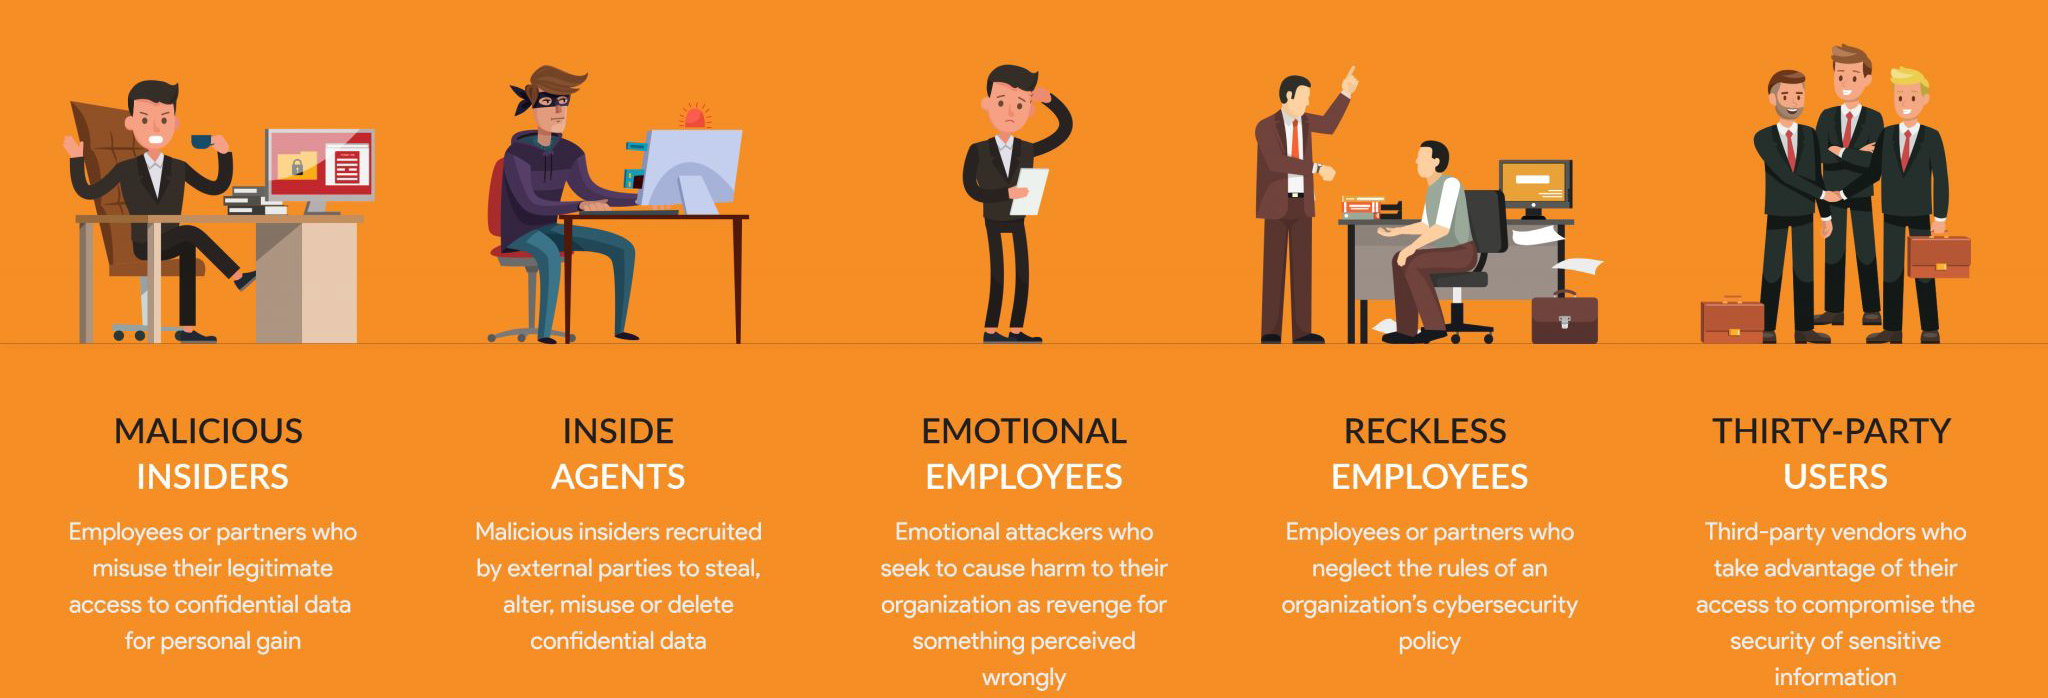
\includegraphics[width=\linewidth]{internaltreaths.png}
            \end{figure}
            A bit more on:
            \begin{itemize}
                \item \textbf{Reckless or socially engineered employees:}   in security we often have a wrong perception of the \textit{human element}.\\
                                                                            When a company gets infected by a malware because a user clicked on a link or something similar, we blame the \textit{stupid} user for it. But, actually it's not fault of the employee: it is fault of who had the responsibility to manage the fact that a threat was present and it had to be controlled.\\
                                                                            Since there will always be someone to click on links, our job is to make sure that they doing it doesn't cause damages to the organization.\\
                                                                            \textit{e.g. in aviation they study human factor to understand what to do to don't let people make mistakes: in airplanes cockpits there are different levers with different shapes, them are exactly shaped the same in different kinds of planes, it is a standard, and the reason is because people lost their lives because of similar levers.}\\
                                                                            The solution wasn't to train pilots, but to make the threat difficult to happen.
                \item \textbf{Thirty-party users:} they're for example consultants that work in a company for a long time, where they actually do jobs very similar to the ones of the actual employees while not being true employees of the company.
            \end{itemize}
\newpage
        \subsection{Data breaches and targeted attacks}
            \begin{figure}[ht!]
                \centering
                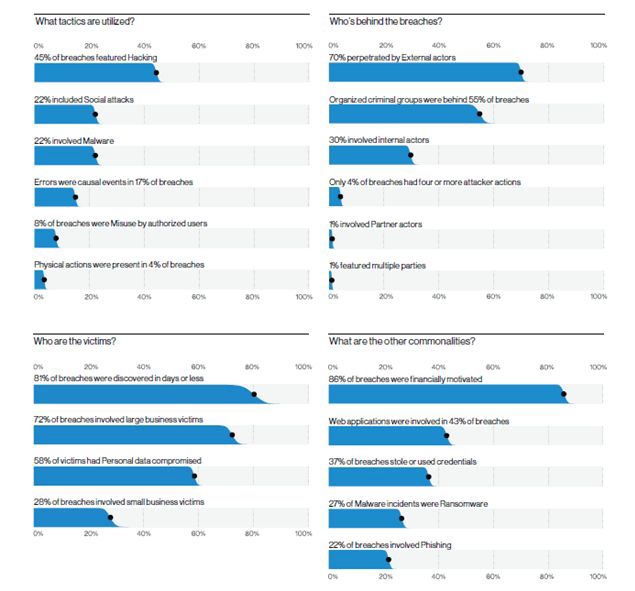
\includegraphics[width=0.7\linewidth]{verizon.png}
            \end{figure}
            Verizon has a big sample of incidents made to their customers:
            \begin{itemize}
                \item The largest part of the attacks features hacking of some sort, the second larger chunk comprends social attacks.
                \item The 70\% of breaches are perpetrated by external actors. This means that 30\% of them starts from the inside, an incredibly high percentage.\\
                      Consider that data are skewed\footnote{biased}, in the real world the internal attacks can be even more! \textit{(remember the external threats reasoning, rationality (data) tells us that a lot of threats come from the inside, while our instinct guide us to be aware of the outside)}
                \item The 86\% of them were financially motivated, 14\% which are not, are a lot too!
            \end{itemize}
            These data are biased and are not representative of the true reality of threats, because simply they're not all collected. This collection can still help us to rationally think on how to manage the overall situation.\\
            Keep in mind that some security incidents are specifically designed to be difficultly found, a lot of them has never been. This means that there is an entire set of breaches that no one ever investigated.\\
            We measure attacks that we investigated/detected, and this is called the \textbf{observation bias}:\\  
            Other attacks by their nature be discovered, \textit{(e.g. Dos, ransomware \dots)} that's the reason why they are so prevalent in our statistics: they are observed.
    \section{Brief history of malicious software}
        \begin{figure}[ht!]
            \centering
            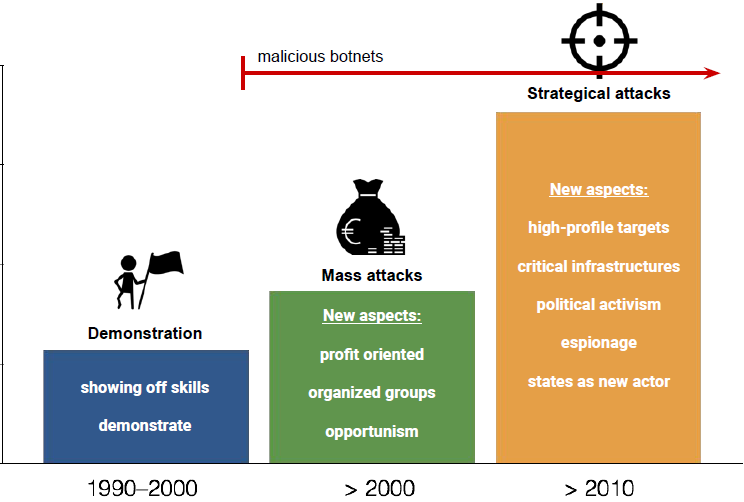
\includegraphics[width=0.7\linewidth]{malicious.png}
        \end{figure}
        Over the last few decades attacks and attackers changed:
        \begin{itemize}
            \item \textbf{1990-2000:} most of the attacks were meant to show skills and explore
            \item \textbf{2000-2010:} with the birth of the Internet, massive, profit oriented attacks born. In this period were born also groups working as profitable enterprises of cybercrime.
            \item \textbf{2010-today:} attacks evolved: mass attacks kept happening, but now a lot of them are high profile financial attacks \textit{(before: ransomwares, i ask small amount of money to single persons. now: ransomware attack specific companies to get a lot of money)} 
        \end{itemize}
\newpage
    \section{Financially motivated attackers}
        Today financially motivated attackers are the "mass", they're interested in monetizing their attacks in possibly two ways:
        \begin{itemize}
            \item \textbf{Direct Monetization:}
                \begin{itemize}
                    \item Credit card/bank account frauds
                    \item Ransomware attacks 
                    \item Fake antiviruses: they show you warnings that say your computer is infected, and to pay to activate the premium version to get rid of the malware. In reality they are just fake programs asking you to pay for a license.
                    \item Premium calls: back in the days when you called to connect to the provider, someone managed to change the number to let you call a costly one.
                \end{itemize} 
            \item \textbf{Indirect Monetization:}
        \end{itemize}
    \section{Ransomwares and ransomware attacks}
        \subsection{Brief history of ransomware}
            \begin{figure}[ht!]
                \centering
                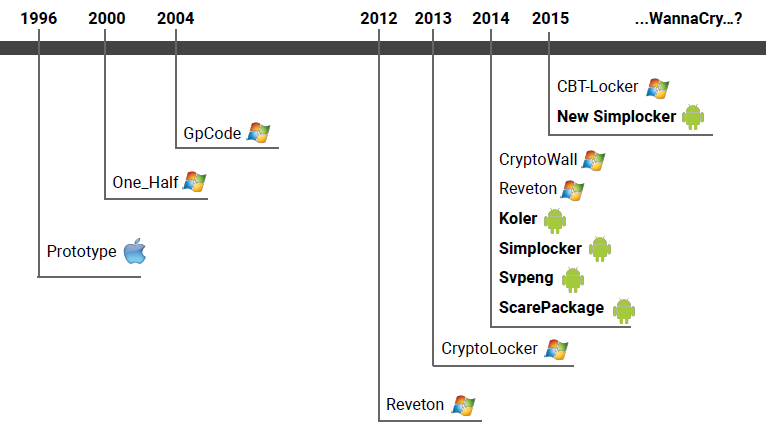
\includegraphics[width=0.40\linewidth]{ransomware_history.png}
            \end{figure}
            In 1996, a paper describing a crypto-malware that was exactly a ransomware was published about 15 years before CryptoLocker which was the first really successful one.\\
            They just \textit{"looked into the crystal ball"} of what in the future would be valuable: taking as hostage digital valuables could become a good way to steal money.\\
            Then something happened:\\
            the internet in 1996 was really different than the one of 2013, ransomwares needed a way for the user to pay a ransom in a way that was easy to perform.
            The preferred way to perform payments on internet is with credit cards, but this kind of payments have two important difects:
            \begin{itemize}
                \item they are trackable
                \item they are refundable when fraudolent
            \end{itemize}
            Then a new suitable way for payments was born: \textbf{cryptocurrencies}.\\
            They perfectly fit this need: they are easily accessible, and payments are not reversible.
%\newpage
        \subsection{Ransomware screenshot and social meanings}
            \begin{figure}[ht!]
                \centering
                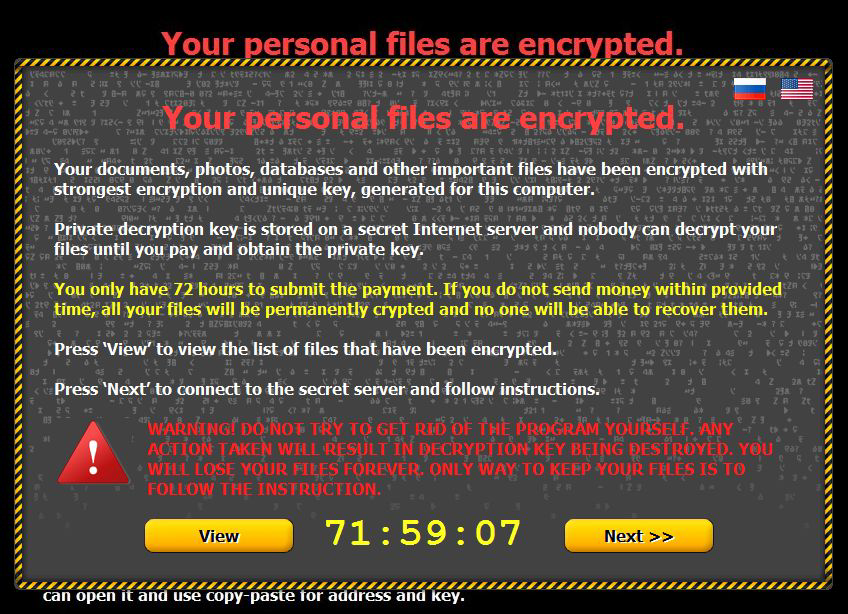
\includegraphics[width=0.40\linewidth]{ransomware_screen.png}
            \end{figure}
            Look at the structure of the timer: it is made to let you to percieve urgency.\\
            The stress of the urgency makes human take bad decisions, with the timer running you're more prone to pay because you feel that you have limited time.\\
            In social engineering attacks, urgency is always an important part. \textit{(think about ultimatums in diplomacy, job offers with time limits, poltrone e sofà...)}
        \subsection{How to get infected}
            \begin{figure}[ht!]
                \centering
                \subfigure[]{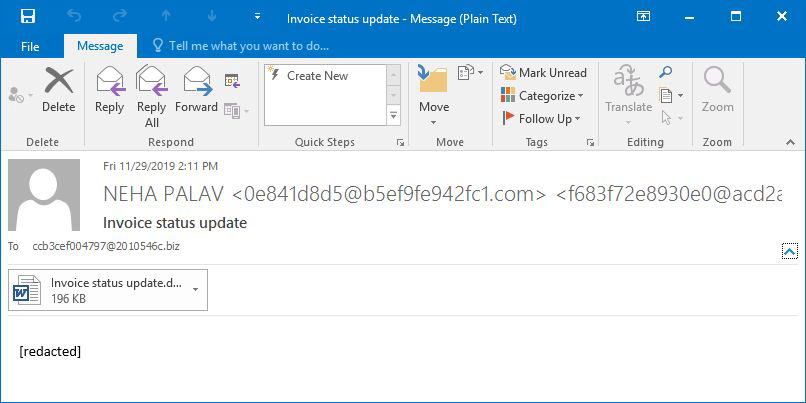
\includegraphics[width=0.48\textwidth]{ransomware_email.png}} 
                \subfigure[]{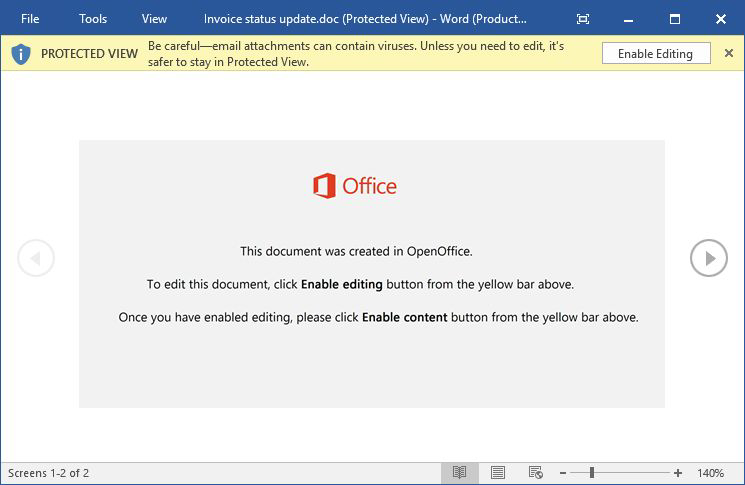
\includegraphics[width=0.48\textwidth]{ransomware_email2.png}} 
            \end{figure}
            Looking at the images we can see an interesting example:
            \begin{itemize}
                \item User receives an e-mail with a short text that contains some sensitive information and an attachment which is social engineered in a way that many people would click
                \item Microsoft Office shows a message to try to prevent code execution, but the user is prone to click "Enable" because the text contained in the document makes him think that's the right thing to do, even if a lot of grammar errors are present and the whole situation looks suspicious
            \end{itemize}
            One could have said that the user must had to be trained to not click, but the reality is that he is not understanding what's happening on his computer.\\
            We can't train a generic user to not click: if your job is to open invoices received by e-mail, there is no way you can be trained.\\
            Even if we train him to click only on what is coming from attendible e-mail addresses, if the \textit{"attendible"} part was hijacked?\\
            What we really should do is to figure out a way that when someone clicks enable, this won't cause any damage. Of course, to train the user to let this happen the less frequent possible is good, but not the main thing to do.